\documentclass{article}\usepackage[]{graphicx}\usepackage[]{color}
%% maxwidth is the original width if it is less than linewidth
%% otherwise use linewidth (to make sure the graphics do not exceed the margin)
\makeatletter
\def\maxwidth{ %
  \ifdim\Gin@nat@width>\linewidth
    \linewidth
  \else
    \Gin@nat@width
  \fi
}
\makeatother

\definecolor{fgcolor}{rgb}{0.345, 0.345, 0.345}
\newcommand{\hlnum}[1]{\textcolor[rgb]{0.686,0.059,0.569}{#1}}%
\newcommand{\hlstr}[1]{\textcolor[rgb]{0.192,0.494,0.8}{#1}}%
\newcommand{\hlcom}[1]{\textcolor[rgb]{0.678,0.584,0.686}{\textit{#1}}}%
\newcommand{\hlopt}[1]{\textcolor[rgb]{0,0,0}{#1}}%
\newcommand{\hlstd}[1]{\textcolor[rgb]{0.345,0.345,0.345}{#1}}%
\newcommand{\hlkwa}[1]{\textcolor[rgb]{0.161,0.373,0.58}{\textbf{#1}}}%
\newcommand{\hlkwb}[1]{\textcolor[rgb]{0.69,0.353,0.396}{#1}}%
\newcommand{\hlkwc}[1]{\textcolor[rgb]{0.333,0.667,0.333}{#1}}%
\newcommand{\hlkwd}[1]{\textcolor[rgb]{0.737,0.353,0.396}{\textbf{#1}}}%

\usepackage{framed}
\makeatletter
\newenvironment{kframe}{%
 \def\at@end@of@kframe{}%
 \ifinner\ifhmode%
  \def\at@end@of@kframe{\end{minipage}}%
  \begin{minipage}{\columnwidth}%
 \fi\fi%
 \def\FrameCommand##1{\hskip\@totalleftmargin \hskip-\fboxsep
 \colorbox{shadecolor}{##1}\hskip-\fboxsep
     % There is no \\@totalrightmargin, so:
     \hskip-\linewidth \hskip-\@totalleftmargin \hskip\columnwidth}%
 \MakeFramed {\advance\hsize-\width
   \@totalleftmargin\z@ \linewidth\hsize
   \@setminipage}}%
 {\par\unskip\endMakeFramed%
 \at@end@of@kframe}
\makeatother

\definecolor{shadecolor}{rgb}{.97, .97, .97}
\definecolor{messagecolor}{rgb}{0, 0, 0}
\definecolor{warningcolor}{rgb}{1, 0, 1}
\definecolor{errorcolor}{rgb}{1, 0, 0}
\newenvironment{knitrout}{}{} % an empty environment to be redefined in TeX

\usepackage{alltt}
\usepackage[letterpaper, total={6in, 8in}]{geometry} %size of paper
\usepackage{indentfirst} %indent after section 
\usepackage{graphicx}
\usepackage{amsmath} %number figure based on subsection also
\numberwithin{figure}{subsection} %number figure based on subsection also
\numberwithin{table}{subsection} %number table based on subsection also
\usepackage{caption}
\captionsetup[figure]{labelfont=bf}
\captionsetup[table]{labelfont=bf,position=below}

\setlength{\parindent}{8ex}
\setlength{\parskip}{2em}
\renewcommand{\baselinestretch}{2.0}
\IfFileExists{upquote.sty}{\usepackage{upquote}}{}
\begin{document}
\setcounter{section}{3} 
\section{Simulation}
\setcounter{subsection}{2}
\subsection{Results for the simulation study}
After repeating sampling with and without replacement, sampling distribution of each candidate estimate can be constructed and their Biase, Variance and MSE can also be obtained. Figure~\ref{fig_dis_size_wr}, Figure~\ref{fig_dis_size_wor}, Table~\ref{tab_size_est} and Table~\ref{tab_per_est} shows that when sampling ``with'' replacement, MLE and Second Order Taylor's Approximation are always the best esitmate for ${\theta}_{A}$ and ${\theta}_{P}$ and when sample size becomes larger, their performance on Variance would also become better. As for the performance of Arithmetric Mean, like our expectation, severely overestimates the true mean no matter how sample size changes. Conversly, when it is sampling ``without'' replacement, the performance of MLE and Second Order Taylor's Approximation estimate are not worse only when the sample size compared to population size is small because when sample size is small, sampling without replacement is similar to sampling with replacement. For Arithmetic Mean, even though its expected value approximates to the true mean as sample size becomes larger, it is still a biased estimate as long as the sample size is not equal to the population size.

To sum up, in this simulation, when it is sampling ``with'' replacement, MLE and the 2nd Order Taylor's Approximation estimate perform best and Arithmetic Mean has the worst performance. Nevertheless, MLE and 2nd Order Taylor's Approximation estimate can only be obtained under strong assumptions on distributions of Area and Circularity. Hence, we also include Weighted Mean in our following distribution for its sufficient performance and its nonparametric assumption. 

\begin{figure}[!htbp]
  \centering
\begin{knitrout}
\definecolor{shadecolor}{rgb}{0.969, 0.969, 0.969}\color{fgcolor}
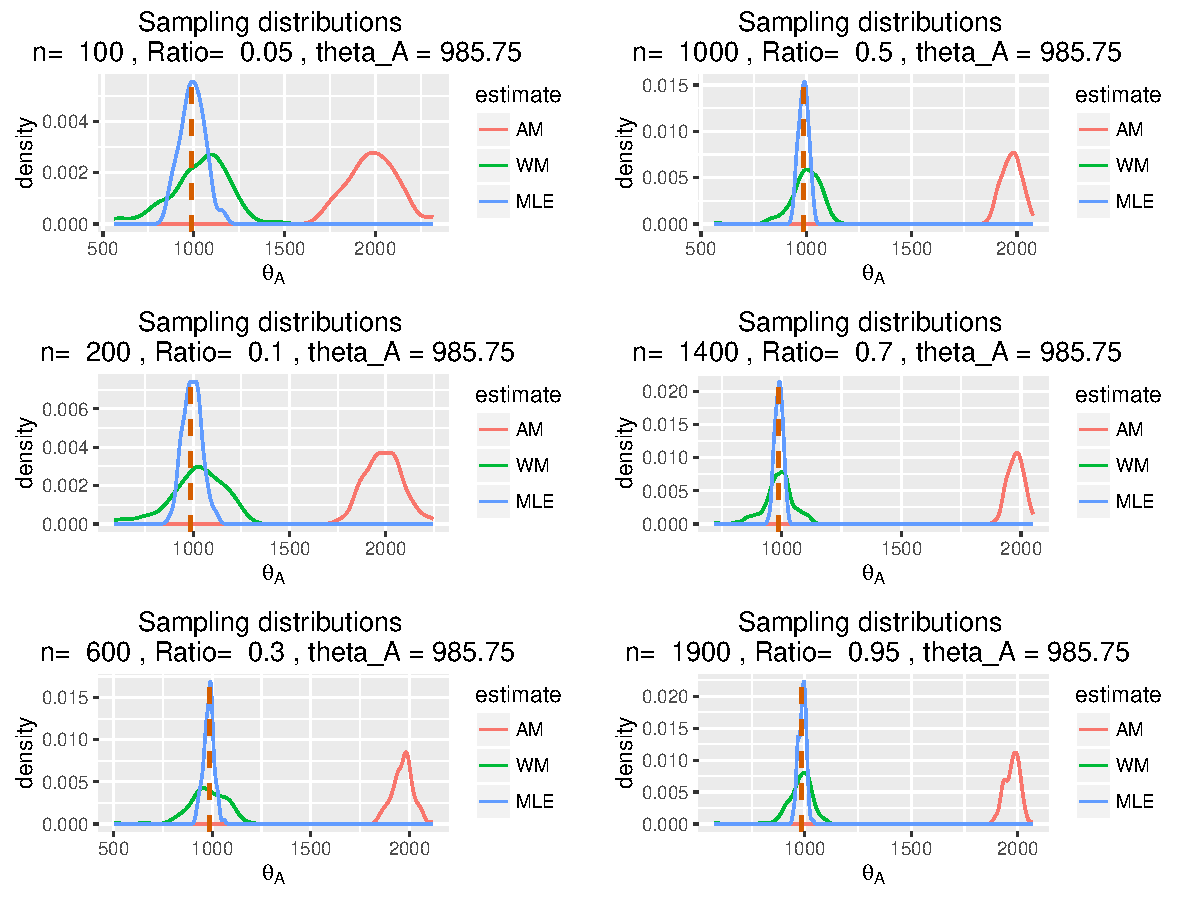
\includegraphics[width=\maxwidth]{figure/unnamed-chunk-1-1} 

\end{knitrout}
\caption{Sampling Distributions for Estimates of Mean Size (WR)}
  \label{fig_dis_size_wr}
\end{figure}




\begin{figure}[!htbp]
  \centering
\begin{knitrout}
\definecolor{shadecolor}{rgb}{0.969, 0.969, 0.969}\color{fgcolor}
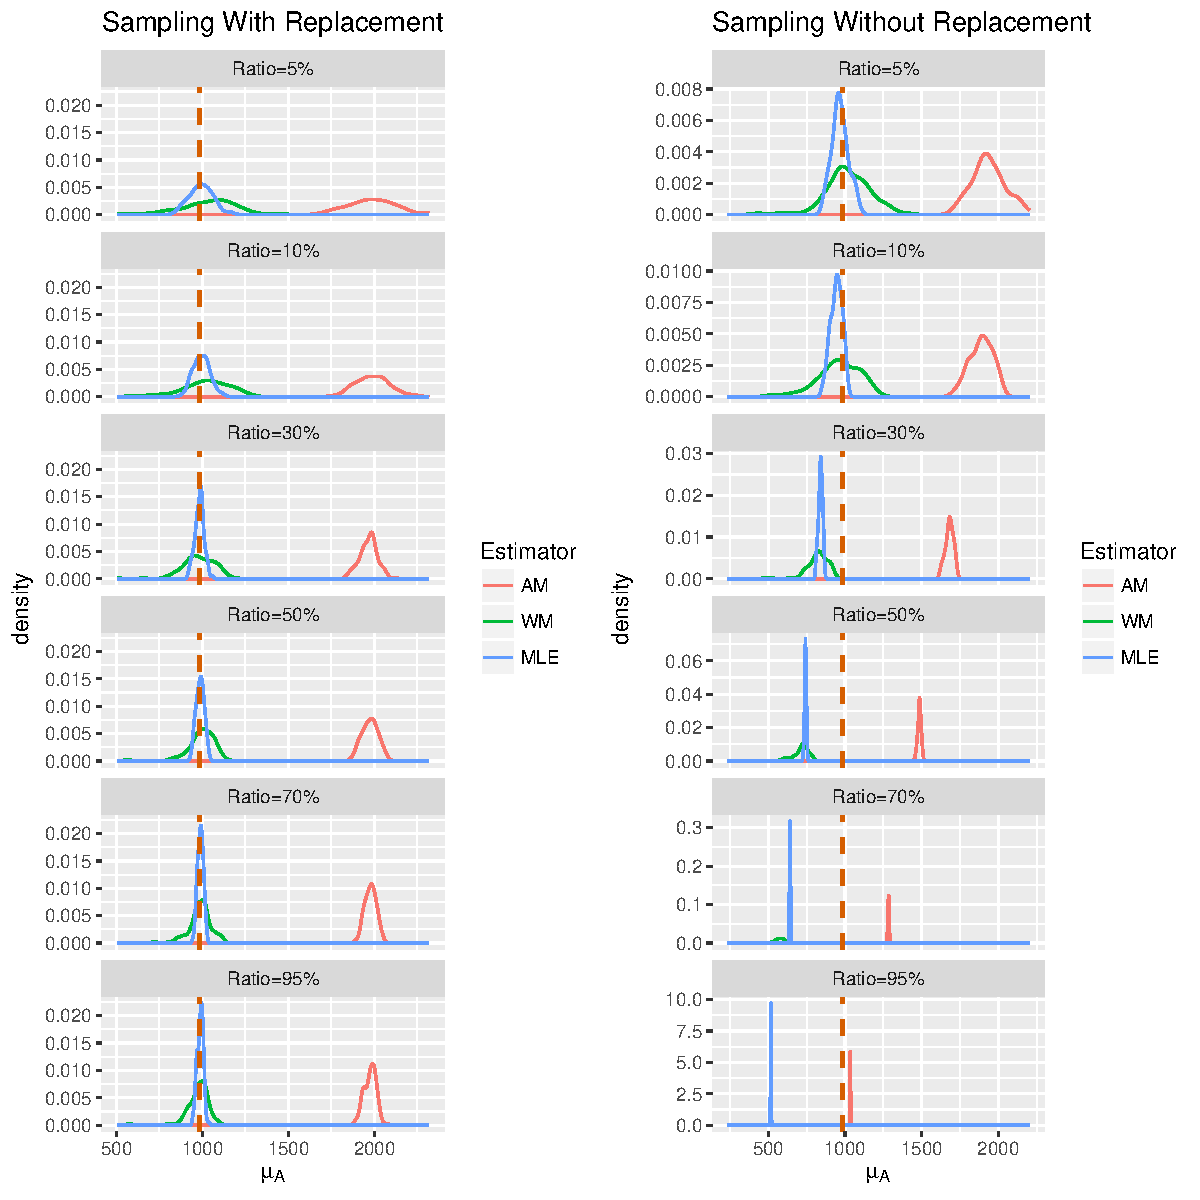
\includegraphics[width=\maxwidth]{figure/unnamed-chunk-3-1} 

\end{knitrout}
\caption{Sampling Distributions for Estimates of Mean Size (WOR)}
  \label{fig_dis_size_wor}
\end{figure}

%latex.default(cbind(t_size_inf, t_size_f), rowname = NULL, file = "",     label = "tab_size_est", col.just = rep("r", 10), caption.loc = c("bottom"),     cgroup = c("Sampling with Replacement", "Sampling without Replacement"),     caption = "Performance Table for Area")%
\begin{table}[!tbp]
\begin{center}
\begin{tabular}{rrrrrcrrrrr}
\hline\hline
\multicolumn{5}{c}{\bfseries Sampling with Replacement}&\multicolumn{1}{c}{\bfseries }&\multicolumn{5}{c}{\bfseries Sampling without Replacement}\tabularnewline
\cline{1-11}
\multicolumn{1}{c}{n}&\multicolumn{1}{c}{Estimate}&\multicolumn{1}{c}{Bias}&\multicolumn{1}{c}{Variance}&\multicolumn{1}{c}{MSE}&\multicolumn{1}{c}{}&\multicolumn{1}{c}{n}&\multicolumn{1}{c}{Estimate}&\multicolumn{1}{c}{Bias}&\multicolumn{1}{c}{Variance}&\multicolumn{1}{c}{MSE}\tabularnewline
\hline
100&AM&1000&17929.4&1017830.2&&100&AM&951.1&11438&916068.9\tabularnewline
&WM&45.2&26254.8&28299.9&&&WM&33.7&22616.9&23753.2\tabularnewline
&MLE&7.1&4482.4&4532.8&&&MLE&-17.3&2859.5&3159.3\tabularnewline
200&AM&1003.9&9268.9&1017014.8&&200&AM&903.1&5635.2&821268.8\tabularnewline
&WM&35&19713.5&20939.4&&&WM&-25.5&18871.3&19523.7\tabularnewline
&MLE&9.1&2317.2&2399.3&&&MLE&-41.3&1408.8&3115.5\tabularnewline
600&AM&980.2&2764.6&963566.6&&600&AM&696&686.8&485126.4\tabularnewline
&WM&-8.7&10112.5&10187.5&&&WM&-163.5&5522.6&32246.4\tabularnewline
&MLE&-2.8&691.2&698.8&&&MLE&-144.9&171.7&21157.8\tabularnewline
1000&AM&988.4&2118.8&979145&&1000&AM&500.3&119.8&250416.6\tabularnewline
&WM&11.2&6076.7&6202.9&&&WM&-274.8&3718&79210.9\tabularnewline
&MLE&1.3&529.7&531.5&&&MLE&-242.7&30&58945.8\tabularnewline
1400&AM&991.7&1100.9&984636.9&&1400&AM&298.4&12.4&89071.2\tabularnewline
&WM&0.9&4239.2&4239.9&&&WM&-416.2&1691.9&174916.1\tabularnewline
&MLE&3&275.2&284.2&&&MLE&-343.7&3.1&118105.7\tabularnewline
1900&AM&989.2&1196.4&979657.2&&1900&AM&49.9&0&2493.2\tabularnewline
&WM&-8.9&4230.7&4310.8&&&WM&-697.6&332.4&486925.7\tabularnewline
&MLE&1.7&299.1&302&&&MLE&-467.9&0&218938.4\tabularnewline
\hline
\end{tabular}

\caption{Performance Table for Area\label{tab_size_est}}\end{center}

\end{table}


\begin{figure}[!htbp]
  \centering
\begin{knitrout}
\definecolor{shadecolor}{rgb}{0.969, 0.969, 0.969}\color{fgcolor}
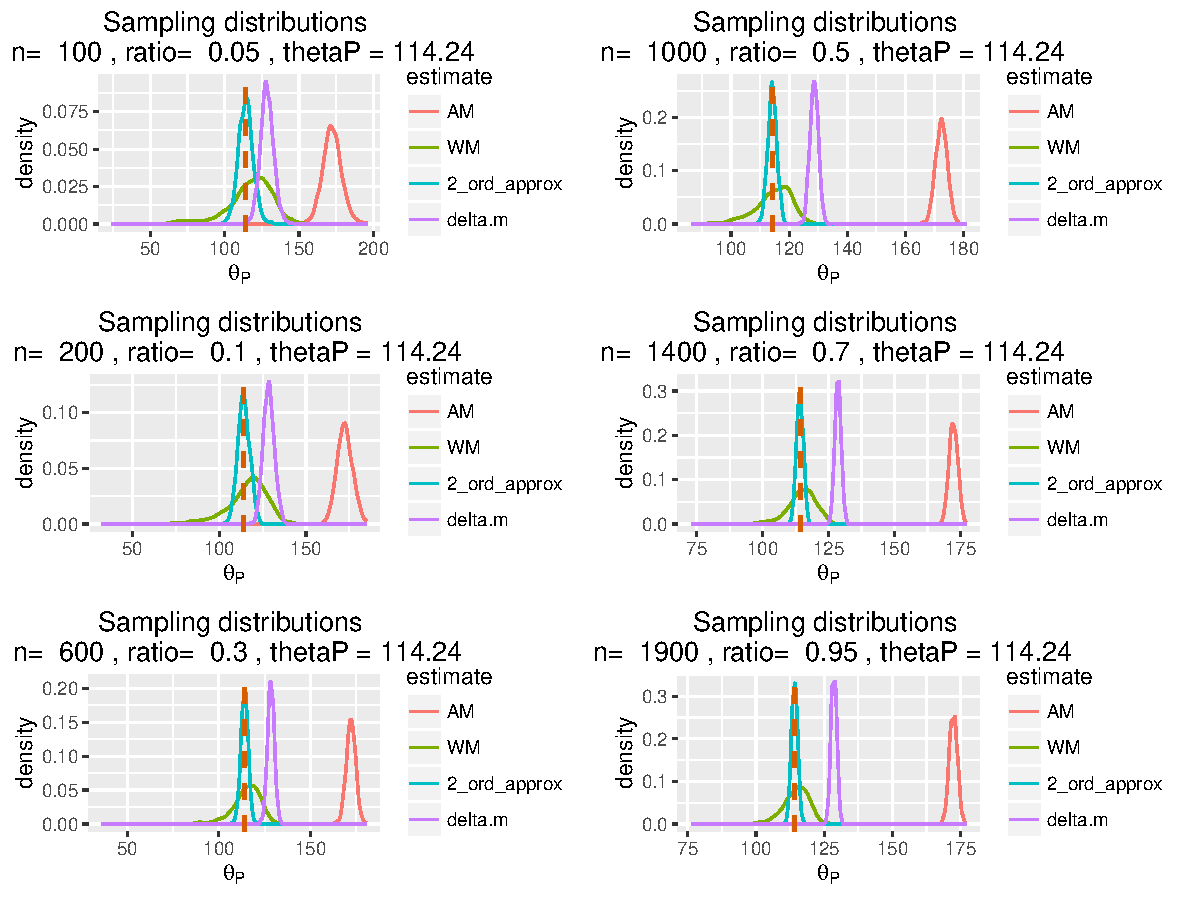
\includegraphics[width=\maxwidth]{figure/unnamed-chunk-5-1} 

\end{knitrout}
\caption{Sampling Distributions for Estimates of Mean Perimeter (WR)}
  \label{fig_dis_per_wr}
\end{figure}

\begin{kframe}


{\ttfamily\noindent\bfseries\color{errorcolor}{\#\# Error in array.mean.per[, 1, i] = apply(sample.mean.per[, , i], 2, mean) - : number of items to replace is not a multiple of replacement length}}\end{kframe}


\begin{figure}[!htbp]
  \centering
\begin{knitrout}
\definecolor{shadecolor}{rgb}{0.969, 0.969, 0.969}\color{fgcolor}
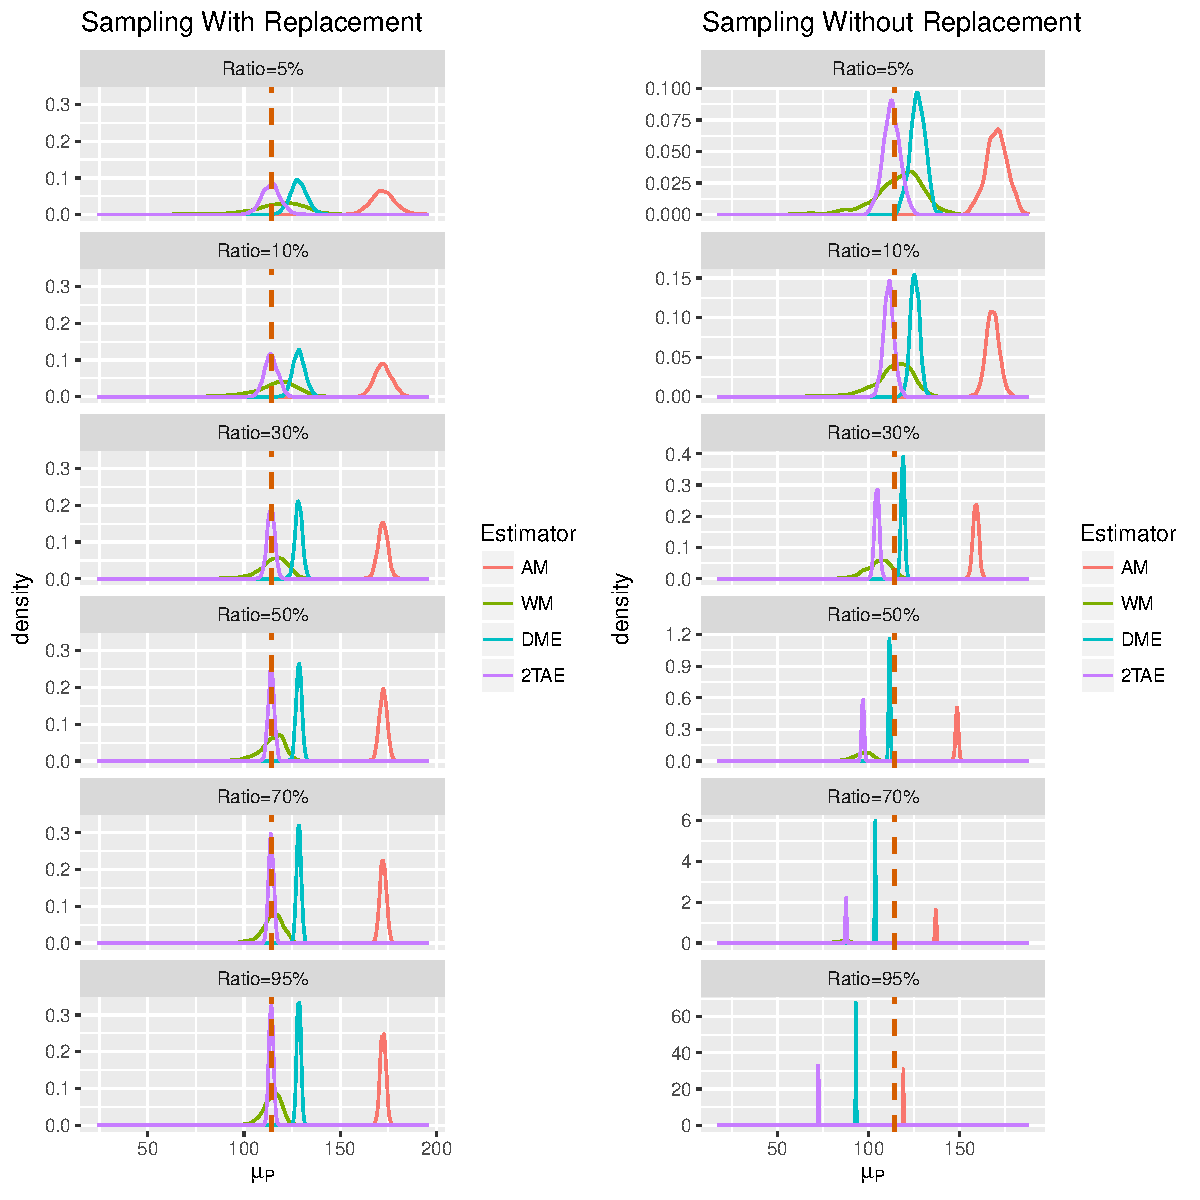
\includegraphics[width=\maxwidth]{figure/unnamed-chunk-7-1} 

\end{knitrout}
\caption{Sampling Distributions for Estimates of Mean Perimeter (WOR)}
  \label{fig_dis_per_wor}
\end{figure}

%latex.default(cbind(t_per_inf, t_per_f), rowname = NULL, file = "",     col.just = rep("r", 10), caption.loc = c("bottom"), label = "tab_per_est",     cgroup = c("Sampling with Replacement", "Sampling without Replacement"),     caption = "Performance Table for Perimeter")%
\begin{table}[!tbp]
\begin{center}
\begin{tabular}{rrrrrcrrrrr}
\hline\hline
\multicolumn{5}{c}{\bfseries Sampling with Replacement}&\multicolumn{1}{c}{\bfseries }&\multicolumn{5}{c}{\bfseries Sampling without Replacement}\tabularnewline
\cline{1-11}
\multicolumn{1}{c}{n}&\multicolumn{1}{c}{Estimate}&\multicolumn{1}{c}{Bias}&\multicolumn{1}{c}{Variance}&\multicolumn{1}{c}{MSE}&\multicolumn{1}{c}{}&\multicolumn{1}{c}{n}&\multicolumn{1}{c}{Estimate}&\multicolumn{1}{c}{Bias}&\multicolumn{1}{c}{Variance}&\multicolumn{1}{c}{MSE}\tabularnewline
\hline
100&AM&$$&$$&$$&&100&AM&56&33.7&3164.6\tabularnewline
&WM&$$&$$&$$&&&WM&1.6&217.9&220.6\tabularnewline
&2nd Approx.&$$&$$&$$&&&2nd Approx.&-1.6&20.9&23.5\tabularnewline
200&AM&$$&$$&$$&&200&AM&53.8&12.8&2905.8\tabularnewline
&WM&$$&$$&$$&&&WM&-0.9&137.1&137.9\tabularnewline
&2nd Approx.&$$&$$&$$&&&2nd Approx.&-3.2&8.1&18.1\tabularnewline
600&AM&$$&$$&$$&&600&AM&44.6&2.4&1992.2\tabularnewline
&WM&$$&$$&$$&&&WM&-9.4&56.6&144.1\tabularnewline
&2nd Approx.&$$&$$&$$&&&2nd Approx.&-9.7&1.7&95.1\tabularnewline
1000&AM&$$&$$&$$&&1000&AM&34.2&0.6&1172.9\tabularnewline
&WM&$$&$$&$$&&&WM&-17.8&32.4&348.5\tabularnewline
&2nd Approx.&$$&$$&$$&&&2nd Approx.&-17.4&0.4&302.4\tabularnewline
1400&AM&$$&$$&$$&&1400&AM&22.6&0.1&511\tabularnewline
&WM&$$&$$&$$&&&WM&-28.7&21.7&845.9\tabularnewline
&2nd Approx.&$$&$$&$$&&&2nd Approx.&-26.6&0.1&710.1\tabularnewline
1900&AM&$$&$$&$$&&1900&AM&4.8&0&23.5\tabularnewline
&WM&$$&$$&$$&&&WM&-58.4&8.1&3420.3\tabularnewline
&2nd Approx.&$$&$$&$$&&&2nd Approx.&-41.8&0&1749.4\tabularnewline
\hline
\end{tabular}

\caption{Performance Table for Perimeter\label{tab_per_est}}\end{center}

\end{table}





\end{document}
